\chapter{Θεωρητικό υπόβαθρο}
?? Στο κεφάλαιο αυτό παρουσιάζονται  αναλυτικά οι τρεις
βασικές τεχνολογίες που έχουν σχέση με την εργασία αυτή, δηλαδή ...

\section{Υπολογιστική Όραση}

Ο άνθρωπος βασίζεται στην αίσθηση της όρασης στην καθημερινή του ζωή. Ο τρόπος με τον οποίο αναλύουμε το περιβάλλον γύρω μας και παίρνουμε αποφάσεις γίνεται ασυναίσθητα. Η υπολογιστική όραση έχει στόχο την δημιουργία συστημάτων που μπορούν να πλοηγούνται στο ίδιο περιβάλλον με εμάς, κάνουν προβλέψεις και παίρνουν αποφάσεις με βάση εικόνες. Ο σχεδιασμός τέτοιων συστημάτων επιτυγχάνεται με αλγόριθμους βαθιάς μάθησης και μηχανικής μάθησης. Αυτοί οι αλγόριθμοι εκπαιδεύονται με μεγάλα σύνολα δεδομένων εικόνων, επιτρέποντας την αναγνώριση προτύπων, αντικειμένων και συνθήκες στο περιβάλλον γύρω τους.

Αν και η μηχανική μάθηση υπάρχει ως αντικείμενο εδώ και πολλά χρόνια, πρόσφατα έχει προσελκύσει έντονο ενδιαφέρον λόγω των σημαντικών προόδων που σημειώθηκαν στην υπολογιστική ισχύ και τη διαθεσιμότητα μεγάλου όγκου δεδομένων για εκπαίδευση.

Σήμερα, εφαρμογές της υπολογιστικής όρασης και των αλγορίθμων βαθιάς μάθησης συναντάμε σε πολλούς τομείς. Αρχικά, επιτρέπει στα ρομπότ να αντιλαμβάνονται οπτικά στοιχεία στο περιβάλλον τους, κρίσιμα για την πλοήγηση τους στον κόσμο μαζί με εμάς. Αλγόριθμους μηχανικής μάθησης και συστήματα τεχνητής νοημοσύνης συναντάμε ακόμη και στα κινητά μας τηλέφωνα. Εφαρμογές επεξεργασίας εικόνων, βελτίωσης των φωτογραφιών, ανίχνευση προσώπων και αναγνώριση κειμένου είναι μόνο μερικά από αυτά.

Ένας από τους πιο σημαντικούς τομείς εφαρμογής είναι η ιατρική, όπου από ιατρικές εικόνες εξάγονται πληροφορίες για τη διάγνωση ενός ασθενούς. Όπως για παράδειγμα η έγκυρη διάγνωση για καρκίνο του μαστού από μαστογραφίες ή ο εντοπισμός όγκου στον εγκέφαλο από μαγνητικές τομογραφίες.

Μια άλλη εφαρμογή της υπολογιστικής όρασης και των αλγόριθμων βαθιάς μάθησης είναι η αυτόνομή οδήγηση. Τα συστήματα αυτά αναγνωρίζουν σήματα, εμπόδια, πεζούς και άλλα οχήματα, αλλά κάνουν και προβλέψεις για την κίνηση αυτών και παίρνουν τις κατάλληλες αποφάσεις για ασφαλή πλοήγηση στους δρόμους.

\section{Πώς ένας υπολογιστής αναγνωρίζει εικόνες}

Ένα από τα βασικά προβλήματα στην Υπολογιστική Όραση είναι αυτό της ταξινόμησης εικόνων. Το πρόβλημα περιλαμβάνει την ανάθεση ετικέτας σε μια εικόνα εισόδου από ένα σταθερό σύνολο κατηγοριών.

Σε αντίθεση με έναν αλγόριθμο που ταξινομεί μια λίστα αριθμών, δεν είναι προφανής ο τρόπος υλοποίησης ενός αλγορίθμου που θα αναγνωρίζει εικόνες. Αντί να προσπαθούμε να προσδιορίσουμε τα χαρακτηριστικά της κάθε κατηγορίας με κώδικα, η προσέγγιση που ακολουθούμε μοιάζει με αυτή που θα ακολουθούσαμε με ένα παιδί. Δίνουμε στον υπολογιστή πολλά παραδείγματα κάθε κατηγορίας και στη συνέχεια αναπτύσσουμε αλγορίθμους μάθησης που εξετάζουν αυτά τα παραδείγματα και μαθαίνουν για την οπτική εμφάνιση κάθε κατηγορίας. Αυτή η προσέγγιση αναφέρεται ως προσέγγιση με βάση τα δεδομένα, καθώς πρώτα συλλέγει δεδομένα από ένα σύνολο κατηγοριοποιημένων δεδομένων.

\subsection{Τι είναι τα Νευρωνικά Δίκτυα?}
Τα νευρωνικά δίκτυα είναι αλγόριθμοι μηχανικής μάθησης εμπνευσμένοι από τον τρόπο λειτουργίας του ανθρώπινου εγκεφάλου. 

Ο εγκέφαλος περιέχει περισσότερα από 80 δισεκατομμύρια κύτταρα - που ονομάζονται νευρώνες - τα οποία ανταλλάσσουν πληροφορίες μεταξύ τους μέσω μικρών παλμών ηλεκτρισμού. Ένας νευρώνας δεν μιλάει απευθείας με όλους τους 80 δισεκατομμύρια άλλους. Αντίθετα, συνδέονται σε δομές που εκτελούν εξειδικευμένες λειτουργίες. Αυτές οι δομές είναι τα βιολογικά νευρωνικά δίκτυα.

Ο ανθρώπινος εγκέφαλος είναι πολύ περίπλοκος, όμως το πιο σημαντικό χαρακτηριστικό που μας ενδιαφέρει είναι η ικανότητα να μαθαίνει από την εμπειρία. Κάθε φορά που μαθαίνουμε κάτι καινούριο, οι νευρώνες στον εγκέφαλό ενισχύουν τις γραμμές επικοινωνίας τους με ορισμένους νευρώνες και αποδυναμώνουν τις συνδέσεις τους με άλλους. Η δομή ενός νευρωνικού δικτύου εξελίσσεται καθώς αποκτάμε νέες ικανότητες. [5]

\subsubsection{Νευρώνας}

Η βασική υπολογιστική μονάδα τον τεχνιτών νευρωνικών δικτύων είναι ο νευρώνας. Οι νευρώνες συνδέονται μεταξύ τους μέσω συνάψεων και σε κάθε σύναψη αντιστοιχεί ένα βάρος \(w_{ij}\), όπου \(j\) είναι ο νευρώνας που στέλνει το σήμα και \(i\) ο νευρώνας που δέχεται το σήμα. Τα σήματα εισόδου που φτάνουν σε έναν νευρώνα μέσω των συνάψεων, πολλαπλασιάζονται με το αντίστοιχο βάρος \(w_{ij}\) και αθροίζονται. Τα βάρη αποτελούν τα εκπαιδεύσιμα στοιχεία των νευρωνικών δικτύων και η τιμή τους έχει να κάνει με το πόσο ένας νευρώνας επηρεάζει έναν άλλο. Εάν το τελικό άθροισμα είναι πάνω από ένα όριο, ο νευρώνας ενεργοποιείται και στέλνει σήμα στην έξοδο. Αυτό μαθηματικά αναπαρίσταται με μία συνάρτηση ενεργοποίησης \(f\), με πιο συνηθισμένη τη σιγμοειδή $\sigma(x) ={1}/{(1 + e^{-x})}$, η οποία περιορίζει τις τιμές στο εύρος από \(0\) έως \(1\). [5]

\begin{Illustration}[!h] 
\centering
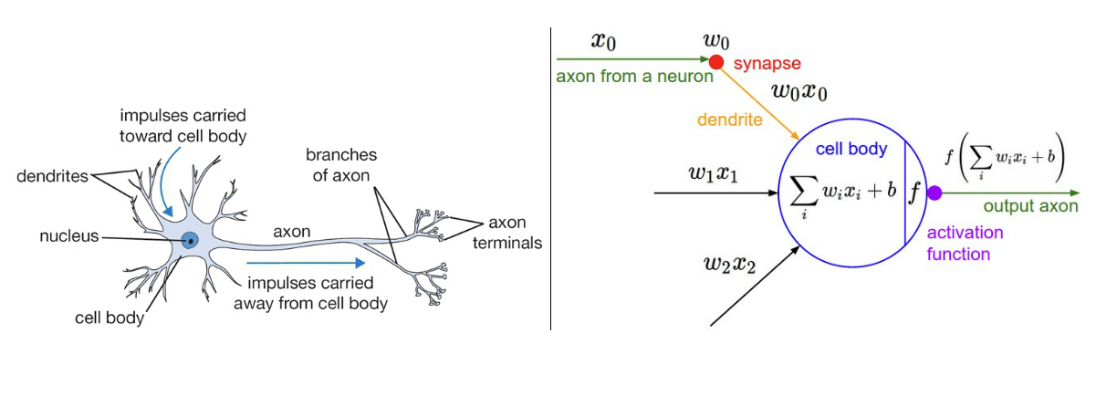
\includegraphics{images/image005.png} 
\caption{Βιολογική και μαθηματική απεικόνιση του νευρώνα [5]} 
\label{neuron-illustration}
\end{Illustration}

\noindent
\begin{minipage}{\textwidth}
\begin{equation}
\hat{x} = \mathbf{x} \mathbf{w} = \sum_{i=1}^{N} x_i w_i + b
\end{equation}

\begin{equation}
y = f(\hat{x})
\end{equation}
\end{minipage}

\subsubsection{Συναρτήσεις Ενεργοποίησης}
Η συνάρτηση ενεργοποίησης, είναι αυτή που εισάγει τη μη γραμμικότητα στο δίκτυο. Χωρίς αυτή ο νευρώνας συμπεριφέρεται σαν γραμμικός ταξινομητής. 

Τα χαρακτηριστικά που θέλουμε να έχει μια συνάρτηση ενεργοποίησης είναι να είναι αύξουσα, να έχει πεπερασμένα απειροστικά όρια, να έχει πεδίο ορισμού το σύνολο των πραγματικών αριθμών και φραγμένο πεδίο τιμών.[6]

Μερικά παραδείγματα συναρτήσεων ενεργοποίησης που συναντάμε φαίνονται παρακάτω:  
 \begin{Illustration}[!h] 
 \centering
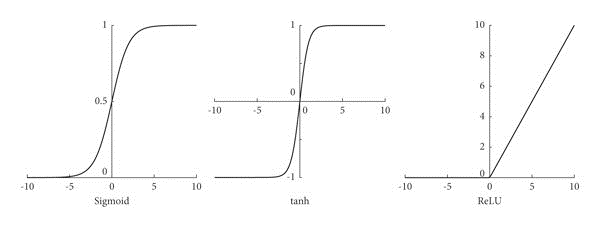
\includegraphics[width=\textwidth]{images/image008.png} \caption{Γραφικές παραστάσεις Σιγμοειδής, Υπερβολική Εφαπτομένη και  \en{ReLU} [7]} 
\label{fig:activation-functions}
\end{Illustration}
\begin{itemize}
\item Σιγμοειδής (\en{Sigmoid})

Η σιγμοειδής συνάρτηση $\sigma(x) ={1}/{(1 + e^{-x})}$, όπως αναφέρθηκε και παραπάνω φράσει την έξοδο ανάμεσα στο $0$ και $1$.  Χρησιμοποιείται συνήθως για μοντέλα όπου η έξοδος εκφράζει πρόβλεψη πιθανότητας. Το μειονέκτημα της  είναι πως ο νευρώνας μπορεί να κορεστεί στο $0$ ή στο $1$, με την παράγωγο να μηδενίζεται σε αυτές τις περιοχές, πράγμα που δημιουργεί πρόβλημα στην διαδικασία της εκπαίδευσης και χρειάζεται προσοχή στην αρχικοποίηση των βαρών. Επιπλέον, η σιγμοειδής δεν έχει κέντρο στο μηδέν, το οποίο μπορεί να προκαλέσει ανεπιθύμητη κίνηση ζιγκ-ζαγκ κατά τις ενημερώσεις των συντελεστών $w$.[5]
\item Υπερβολική εφαπτομένη –  \en{Tanh}

Η υπερβολική εφαπτομένη έχει πεδίο τιμών το $[-1,1]$. Όπως και στην σιγμοειδή, οι νευρώνες μπορεί να κορεστούν, όμως έχει κέντρο το $0$. 
\[
\tanh(x) = \frac{e^x - e^{-x}}{e^x + e^{-x}}
\]

\item Ανορθωμένη γραμμική συνάρτηση - \en{ReLU  (Rectified Linear Unit)}

Η \en{ReLU} όπως φαίνεται από τον τύπο, είναι ένα κατώφλι στο μηδέν
\[
f(x) = \max(0, x) = 
\begin{cases} 
x & \text{\en{if} } x \geq 0 \\
0 & \text{\en{if} } x < 0 
\end{cases}
\]
Χρησιμοποιείται στα νευρωνικά δίκτυα πολλών επιπέδων καθώς φαίνεται να επιταχύνει κατά πολύ την σύγκλιση του αλγόριθμου εκπαίδευσης στοχαστικής καθόδου με βάση την κλίση \en{(stochastic gradient descent)} σε σχέση με την υπερβολική εφαπτομένη και τη σιγμοειδή. Επιπλέον, στον υπολογισμό της είναι πολύ απλή σε σχέση με συναρτήσεις που περιέχουν εκθετικά. Το μειονέκτημα της είναι πώς η μηδενική πλευρά έχει παραγωγό 0 και κατά την εκπαιδεύσει μπορεί κάποιοι νευρώνες να μην ενεργοποιηθούν ποτέ.
\end{itemize}

\subsection{Δομή νευρωνικού δικτύου}
Τα Νευρωνικά δίκτυα οργανώνονται σε επίπεδα από νευρώνες. Ένα επίπεδο εισόδου, ένα ή παραπάνω ενδιάμεσα κρυφά επίπεδα, και ένα επίπεδο εξόδου [8]. Ο πιο συνηθισμένος τρόπος διασύνδεσης των επιπέδων είναι το πλήρως διασυνδεμένο επίπεδο, όπου κάθε νευρώνας συνδέεται με τους νευρώνες του επόμενου επιπέδου και οι έξοδοι των νευρώνων του ενός επιπέδου γίνονται είσοδος του επόμενου, χωρίς όμως να έχουμε διασυνδέσεις μεταξύ νευρώνων του ίδιου επιπέδου.  

%  \begin{figure}[!ht] \centering
% 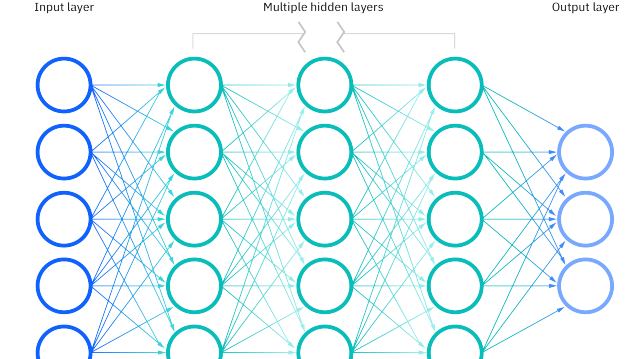
\includegraphics[width=\textwidth]{images/image012.png} \caption{Πλήρως διασυνδεμένο νευρωνικό δίκτυο [8]} 
% \label{fig:fc-network}
% \end{figure} 
\begin{Illustration}[!h] 
	\centering
	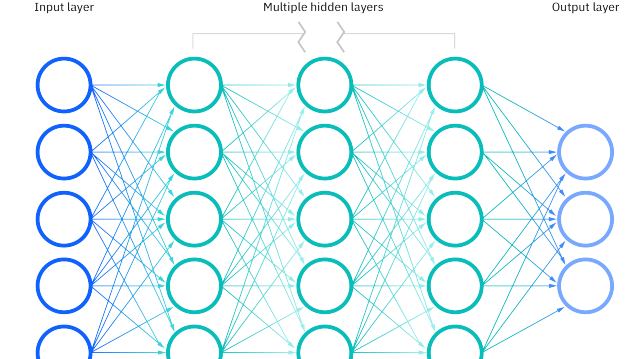
\includegraphics[width=0.6\textwidth]{images/image012.png} \caption{Πλήρως διασυνδεμένο νευρωνικό δίκτυο [8]} 
	\label{fc-network}
\end{Illustration}


Στο επίπεδο εισόδου τροφοδοτούμε τα δεδομένα τα οποία θα παράγουν μια έξοδο. Τα ενδιάμεσα επίπεδα ανάλογα με το είδος του επιπέδου εκτελούν υπολογισμούς και πράξεις στα δεδομένα. Προσθέτοντας επίπεδα αυξάνεται ο βαθμός ελευθερίας του νευρωνικού δικτύου και μπορεί να αναγνωρίσει πιο περίπλοκα μοτίβα και χαρακτηριστικά στα δεδομένα. Βαθιά νευρωνικά δίκτυα είναι αυτά που αποτελούνται από ένα μεγάλο αριθμό κρυφών επιπέδων. Το επίπεδο εξόδου συνήθως είναι ένας αριθμός που αντιπροσωπεύει τις βαθμολογίες των κλάσεων ταξινόμησης.

\subsection{Εκπαίδευση Νευρωνικών Δικτύων}

\subsubsection{Οπισθοδρομική Διάδοση - \en{Backpropagation}}

Κύριος στόχος της εκπαίδευσης ενός νευρωνικού δικτύου είναι η προσαρμογή των παραμέτρων του δικτύου ώστε να δίνουν όσο το δυνατόν πιο ακριβή αποτελέσματα για κάθε είσοδο. 

Αρχικά θέτονται τυχαίες τιμές στα βάρη του νευρωνικού και υπολογίζεται η έξοδος για μια είσοδο. Υπολογίζεται η διαφορά με την τιμή που θα περιμέναμε να έχει η έξοδος μέσο μιας συνάρτησης σφάλματος. Στόχος είναι η ελαχιστοποίηση του σφάλματος μεταβάλλοντας τα βάρη.

Η οπισθοδρομική διάδοση είναι η τεχνική που χρησιμοποιούμε για να βρούμε τα βέλτιστα βάρη, και αναφέρεται στη διάδοση αυτού του σφάλματος από την έξοδο στην είσοδο του δικτύου, υπολογίζοντας τις παραγώγους για την αναπροσαρμογή των παραμέτρων. Η διαδικασία αυτή γίνεται επαναληπτικά για πολλά δεδομένα έως ότου υπάρξει κάποια σύγκλιση.[9]

??Σε αυτή τη διπλωματική δεν θα ασχοληθούμε με το κομμάτι της εκπαίδευσης.

\subsection{Συνελικτικά Νευρωνικά Δίκτυα}

Τα συνελικτικά νευρωνικά δίκτυα \en{(Convolutional Neural Networks – CNN)}  είναι μια κατηγορία νευρωνικών δικτύων τα οποία χρησιμοποιούνται κυρίως στην υπολογιστική όραση καθώς έχουν πολύ καλή απόδοση σε δεδομένα που έχουν κάποια χωρική διάταξη, όπως οι εικόνες.

Τα συνελικτικά νευρωνικά δίκτυα είναι όμοια με τα πλήρως διασυνδεμένα νευρωνικά δίκτυα με τη διαφορά ότι αντί για νευρώνες έχουμε φίλτρα ή αλλιώς πυρήνες τα οποία εκτελούν τη μαθηματική πράξη της συνέλιξης. Τα φίλτρα είναι δισδιάστατοι πίνακες με εκπαιδεύσιμα βάρη με τα οποία σαρώνουμε τα δεδομένα εισόδου, δηλαδή τις εικόνες, για να εξάγουμε χαρακτηριστικά από αυτές. 

Εάν τροφοδοτήσουμε ένα πλήρως διασυνδεμένο νευρωνικό δίκτυο με μία εικόνα, κάθε πίξελ της εικόνας στην είσοδο συνδέεται με κάθε νευρώνα του κρυφού επιπέδου. Αρχικά, η δισδιάστατη εικόνα έχει μετατραπεί σε ένα μονοδιάστατο διάνυσμα με αποτέλεσμα να χάνεται κάθε χωρική πληροφορία που υπάρχει σε αυτή. Επιπλέον, για μία εικόνα $100\times100$ πίξελ, η οποία θεωρείται μικρή για τα σημερινά δεδομένα, χρειαζόμαστε 10.000 παραμέτρους για κάθε νευρώνα του κρυφού επιπέδου, πράγμα που αυξάνει πάρα πολύ τον αριθμό τον παραμέτρων του δικτύου.  Άρα, το πλήρως διασυνδεμένο νευρωνικό δίκτυο δεν αποτελεί καλό τρόπο επίλυσης του προβλήματος της αναγνώρισης εικόνων.

Χρησιμοποιώντας φίλτρα, κάθε νευρώνας βλέπει ένα μέρος της εικόνας και μας δίνει μία έξοδο που αντιστοιχεί σε αυτό το κομμάτι. Ολισθαίνοντας το φίλτρο σε όλη την εικόνα,  παίρνουμε σαν έξοδο μια άλλη εικόνα την οποία τροφοδοτούμε σε επόμενο επίπεδο. Με αυτό τον τρόπο έχουμε καταφέρει να διατηρήσουμε την χωρική πληροφορία που περιέχεται στην είσοδο μας και εκπαιδεύοντας τα βάρη στα φίλτρα, το δίκτυο μαθαίνει  να εντοπίζει χαρακτηριστικά και μοτίβα στις εικόνες. Επιπλέον, χρησιμοποιούμε τα ίδια βάρη για μια εικόνα, πράγμα  που μειώνει  το πλήθος των παραμέτρων του δικτύου.

Η πράξη της συνέλιξης μας δείχνει πόσο  κοντά είναι η εικόνα στο μοτίβο ή το χαρακτηριστικό στοιχείο που ψάχνουμε. Η εικόνα που παίρνουμε σαν αποτέλεσμα είναι μια απεικόνιση των χαρακτηριστικών \en{(feature map)}. Χρησιμοποιώντας πολλά φίλτρα μπορούμε να εξάγουμε διαφορετικά χαρακτηριστικά από την εικόνα. Με κάθε επίπεδο που προστίθεται το δίκτυο αυξάνει την πολυπλοκότητά του και αναγνωρίζει μεγαλύτερα τμήματα της εικόνας. Τα πρώτα επίπεδα επικεντρώνονται σε απλά χαρακτηριστικά, όπως χρώματα και ακμές. Καθώς η εικόνα επεξεργάζεται από τα διάφορα επίπεδα, το δίκτυο αρχίζει να αναγνωρίζει μεγαλύτερα στοιχεία της εικόνας ή σχήματα αντικειμένων έως ότου τελικά αναγνωρίσει το εικονιζόμενο αντικείμενο. [5], [8], [10], [11]
 
\begin{Illustration}[!ht] \centering
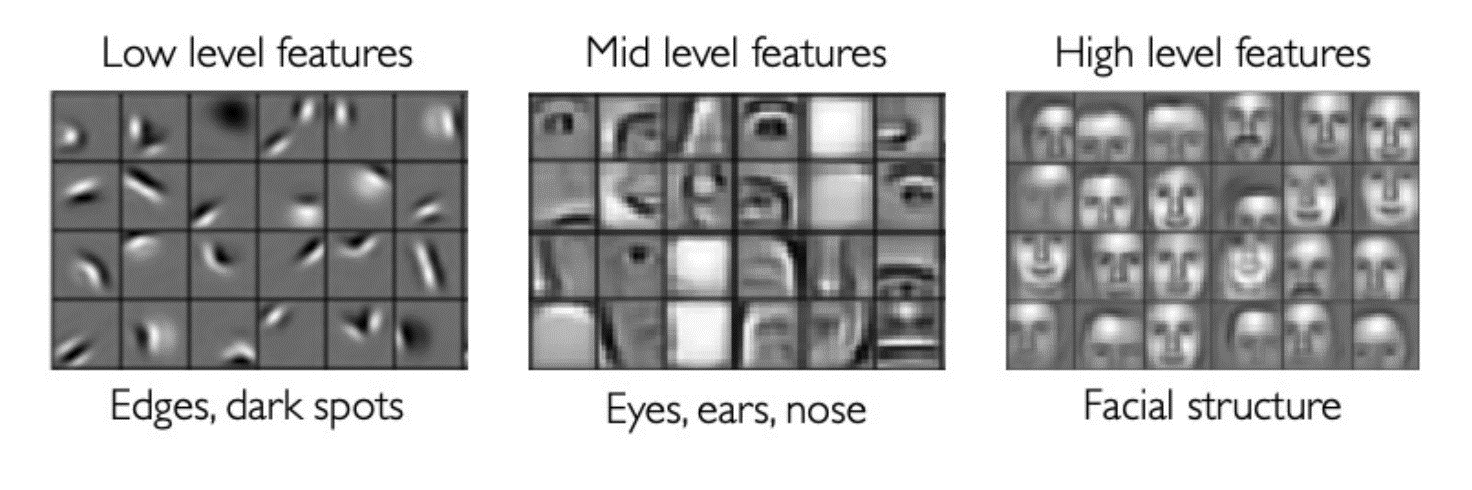
\includegraphics[width=\textwidth]{images/image014.png} \caption{Απεικόνιση χαρακτηριστικών που εξάγει το νευρωνικό δίκτυο στα επίπεδα  [10]} 
\label{fig:feature-exptraction}
\end{Illustration} 

\subsection{Επίπεδα Συνελικτικών Νευρωνικών Δικτύων}

Τα συνελικτικά νευρωνικά δίκτυα αποτελούνται από τρείς τύπους επιπέδων. Το συνελικτικό επίπεδο ακολουθούμενο από μια μη γραμμικότητα, το επίπεδο δειγματοληψίας και το πλήρως διασυνδεμένο επίπεδο. Μια απλή αρχιτεκτονική συνελικτικού δικτύου είναι η εξής:

\begin{enumerate}
    \item Το \textbf{επίπεδο εισόδου} είναι αυτό στο οποίο τροφοδοτούνται τα δεδομένα σε μορφή τρισδιάστατων πινάκων, για έγχρωμες εικόνες πλάτος, ύψος και τρία χρωματικά κανάλια \en{RGB}.
    \item \textbf{Συνελικτικό επίπεδο} \en{(convolution layer)} ακολουθούμενο από μία μη γραμμικότητα, συνήθως \en{ReLU}. Υπολογίζεται η συνέλιξη της εικόνας εισόδου με τα φίλτρα, και στη συνέχεια εφαρμόζεται η συνάρτηση ενεργοποίησης \en{ReLU} για κάθε στοιχείο της εξόδου.
    \item Tο \textbf{επίπεδο δειγματοληψίας} \en{(pooling layer)} είναι μία πράξη υποδειγματοληψίας που εφαρμόζουμε ώστε να μειώσουμε τη διάσταση των δεδομένων.
    \item Το \textbf{πλήρες διασυνδεμένο επίπεδο} \en{(fully connected layer)} είναι αυτό που κάνει την ταξινόμηση και μας δίνει την βαθμολογία της κάθε κλάσης.
\end{enumerate}

\begin{Illustration}[!ht] \centering
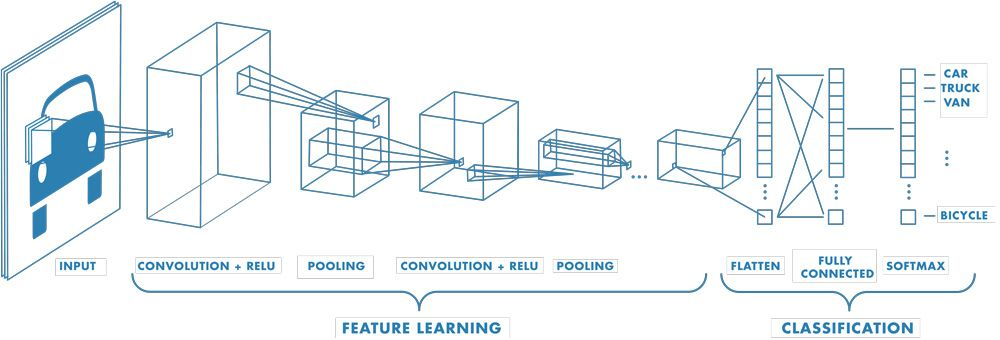
\includegraphics[width=\textwidth]{images/image015.jpg} \caption{Αρχιτεκτονκική συνελικτικού νευρωνικού δικτύου  [12]} 
\label{fig:}
\end{Illustration} 
